\documentclass[
    10pt,
    a4paper,
    oneside,
    headinclude,footinclude,
    BCOR=5mm,
    captions=tableabove
]{scrartcl}

%%%%%%%%%%%%%%%%%%%%%%%%%%%%%%%%%%%%%%%%%
% Arsclassica Article
% Structure Specification File
%
% This file has been downloaded from:
% http://www.LaTeXTemplates.com
%
% Original author:
% Lorenzo Pantieri (http://www.lorenzopantieri.net) with extensive modifications by:
% Vel (vel@latextemplates.com)
%
% License:
% CC BY-NC-SA 3.0 (http://creativecommons.org/licenses/by-nc-sa/3.0/)
%
%%%%%%%%%%%%%%%%%%%%%%%%%%%%%%%%%%%%%%%%%

%----------------------------------------------------------------------------------------
%	REQUIRED PACKAGES
%----------------------------------------------------------------------------------------

\usepackage[
nochapters, % Turn off chapters since this is an article        
beramono, % Use the Bera Mono font for monospaced text (\texttt)
eulermath,% Use the Euler font for mathematics
pdfspacing, % Makes use of pdftex’ letter spacing capabilities via the microtype package
dottedtoc % Dotted lines leading to the page numbers in the table of contents
]{classicthesis} % The layout is based on the Classic Thesis style

\usepackage{arsclassica} % Modifies the Classic Thesis package

\usepackage[T1]{fontenc} % Use 8-bit encoding that has 256 glyphs

\usepackage[utf8]{inputenc} % Required for including letters with accents

\usepackage{graphicx} % Required for including images
\graphicspath{{Figures/}} % Set the default folder for images

\usepackage{enumitem} % Required for manipulating the whitespace between and within lists

\usepackage{lipsum} % Used for inserting dummy 'Lorem ipsum' text into the template

\usepackage{subfig} % Required for creating figures with multiple parts (subfigures)

\usepackage{amsmath,amssymb,amsthm} % For including math equations, theorems, symbols, etc

\usepackage{varioref} % More descriptive referencing

%----------------------------------------------------------------------------------------
%	THEOREM STYLES
%---------------------------------------------------------------------------------------

\theoremstyle{definition} % Define theorem styles here based on the definition style (used for definitions and examples)
\newtheorem{definition}{Definition}

\theoremstyle{plain} % Define theorem styles here based on the plain style (used for theorems, lemmas, propositions)
\newtheorem{theorem}{Theorem}

\theoremstyle{remark} % Define theorem styles here based on the remark style (used for remarks and notes)

%----------------------------------------------------------------------------------------
%	HYPERLINKS
%---------------------------------------------------------------------------------------

\hypersetup{
%draft, % Uncomment to remove all links (useful for printing in black and white)
colorlinks=true, breaklinks=true, bookmarks=true,bookmarksnumbered,
urlcolor=webbrown, linkcolor=RoyalBlue, citecolor=webgreen, % Link colors
pdftitle={}, % PDF title
pdfauthor={\textcopyright}, % PDF Author
pdfsubject={}, % PDF Subject
pdfkeywords={}, % PDF Keywords
pdfcreator={pdfLaTeX}, % PDF Creator
pdfproducer={LaTeX with hyperref and ClassicThesis} % PDF producer
}
\usepackage[utf8]{inputenc}
\usepackage[french]{babel}
\usepackage[T1]{fontenc}
\usepackage{amsmath}
\usepackage{amsfonts}
\usepackage{amssymb}
\hyphenation{Fortran hy-phe-ation}

\usepackage{graphicx}
\usepackage{here}
\usepackage{subfig}
\captionsetup{figurename=Figure,margin=1cm,format=hang,font=small,format=plain,labelfont={bf,up},textfont={it}}
\captionsetup[subfigure]{margin=0cm,font=small,format=plain,labelfont={bf,up},textfont={up}}


\title{\normalfont{\spacedallcaps{Ready-Player-One}}}
\subtitle{Rapport du groupe Harpon}

\author{Martin Lehoux, Pierre Biret \and Sacha Seksik, Loïc Audoin}
\date{\today}

\begin{document}
    
\renewcommand{\sectionmark}[1]{\markright{\spacedlowsmallcaps{#1}}}
\lehead{\mbox{\llap{\small\thepage\kern1em\color{halfgray} \vline}\color{halfgray}\hspace{0.5em}\rightmark\hfil}}
\pagestyle{scrheadings}

\maketitle
% \setcounter{tocdepth}{2}
% \tableofcontents
% \listoffigures
% \listoftables

\section*{Abstract}
Le projet "Ready player one", constitué de deux équipes (Harpon et Eponge) a pour but l'apprentissage par un réseau de neurones d'une stratégie gagnante au jeu "Pong" sur Atari.

L'interêt du projet étant la compréhension des mécanismes des réseaux de neurones par l'ensemble des étudiants, ce projet sera donc constitué de plusieurs parties qui mèneront à terme à la réalisation du projet.



\newpage
\section{Réalisation du perceptron}


\subsection{premières approches}

la première étape de notre projet conserne la création d'un perceptron (ou MLP). pour cela, nous avons d'abord eu une approche théorique, afin de comprendre ce qu'était un réseau de neurones au niveau mathématique et en quoi il pouvait présenter une solution pour résoudre numériquement un problème de classification dans un espace à n dimensions. Pour celà, nous nous sommes évidemment appuyés sur les travaux fondateur de Yann LeCun, et ceux-ci nous serviront régulièrement par la suite. 

L'important a été de comprendre en quoi la minimisation d'une fonction d'erreur était faisable en temps fini. Pour celà on s'interesse à la fonction associant un vecteur d'entrée et les paramètres (Poids, Biais) liés à chaque neurone à un vecteur de sortie du réseaux de neurones. Cette opération complexe est réalisées par applications successives des fonctions d'activations liées à chaque couche de neurones aux résultats (pondérés par des poids et biais) de la couche précédentes. 
Le calcul de cette fonction est noté dans ce futur rapport comme frontpropagation ou propagation directe.

 La fonction d'erreur mentionnée plus haut représentant la distance entre les sorties de la frontpropagations pour un vecteur d'entrées et les sorties voulues pour cette entrée, le principe du réseau de neurone va être de minimiser cette erreur en utilisant sa dérivée par rapports au différents paramètres du réseau. On remarque rapidement que le calcul d'une dérivée par rapport à un poids ou biais associé à un neurone d'une couche donnée va faire intervenir toutes les dérivées par rapports aux couches suivantes. le calcul de la déroulée va donc se faire dans le sens indirect, d'où l'usage du terme backpropagation.

De plus, il est utile de comprendre que les fonction d'activation choisies auront la propriété utile de permettre en temps réduit le calcul de leur dérivée en fonction de leur résultat : on a pour tout $x$, $f'(x)=G(f(x))$ , ce qui va permettre, en retenant les résultats de chaque neurone pour la propagation directe, d'effectuer rapidement la propagation indirecte. 

Enfin, le processus de minimisation se fait par des méthodes basés sur la méthode du gradient vectoriel:

 \hspace{4mm} $Sys(n+1) = Sys(n) - Erreur[Syst(n)] \times Jacobienne(Erreur[Sys(n)]) ^{-1} $   

L'algorithme donc dépendre, en plus du choix de la fonction de coût et de la fonction d'activation des neurones, du choix de la méthode de minimisation et de ses paramètres associés (learning rate).
\vspace{5mm}

Avant de commencer la programmation d'un perceptron, il a fallu commencer par comprendre le fonctionnement opération par opération d'un neurone. Une feuille de calcul a donc été mise en place pour calculer à la main une itération de l'apprentissage d'un réseau de neurones de la fonction XOR à deux entrées avec rétropropagation, après visualisation par tous les étudiants du groupe d'une vidéo très bien réalisée sur le fonctionnement des réseaux neuronaux.

La mise en place de cette feuille de calcul a mis en évidence la complexité des opérations effectuées par les réseaux de neurones, ainsi que l'impossibilité d'effectuer tous les calculs à la main. Toutefois ce premier exemple de réseaux a permis à l'ensemble de l'équipe de comprendre comment se comportait un réseau de neurones à plusieurs couches, et leur a permis de se lancer dans le vif du sujet. 
\vspace{30mm}

\begin{figure}[!h]
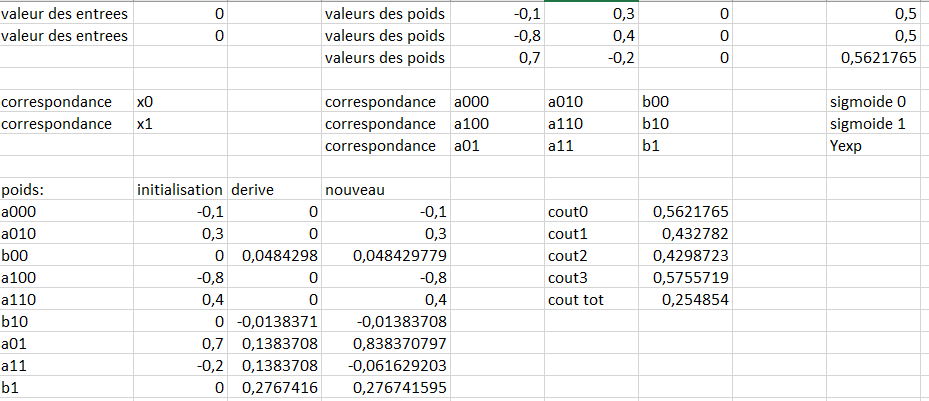
\includegraphics[width=\linewidth]{excelXOR.png}
\centering
 \caption{modélisation d'un apprentissage sur une entrée pour un réseau 2-2-1 sur Excel}
 \label{fig:excelXOR}
\end{figure}
\vspace{5mm}
L'étape suivante fut donc la programmation en Python d'un réseau de neurones, celle-ci reposant sur la dualité entre parcours du réseau direct pour les calculs et inverse pour l'apprentissage (frontpropagation et backpropagation). La première difficulté rencontrée lors de la programmation a été la lenteur de nos algorithmes. En effet, des calculs qui auraient pu être effectués matriciellement (multiplication d'une couche par une matrice de poids et ajout de la matrice de biais pour obtenir l'entrée de la couche de neurones suivantes) étaient réalisés ligne par ligne à travers des listes. Le module numpy a donc été utilisé pour optimiser les calculs matriciels, améliorant la vitesse de calcul, comme on le voit sur la première courbe. L'utilisation de numpy, non essentielle pour nos premiers perceptrons approximants la fonctions XOR, fut nécessaire à l'apprentissage de réseaux plus grands, en particulier dans notre application suivante à la base de données MNIST pour lesquels les calculs passèrent de l'ordre de l'heure à la minute.

\begin{figure}[h!]
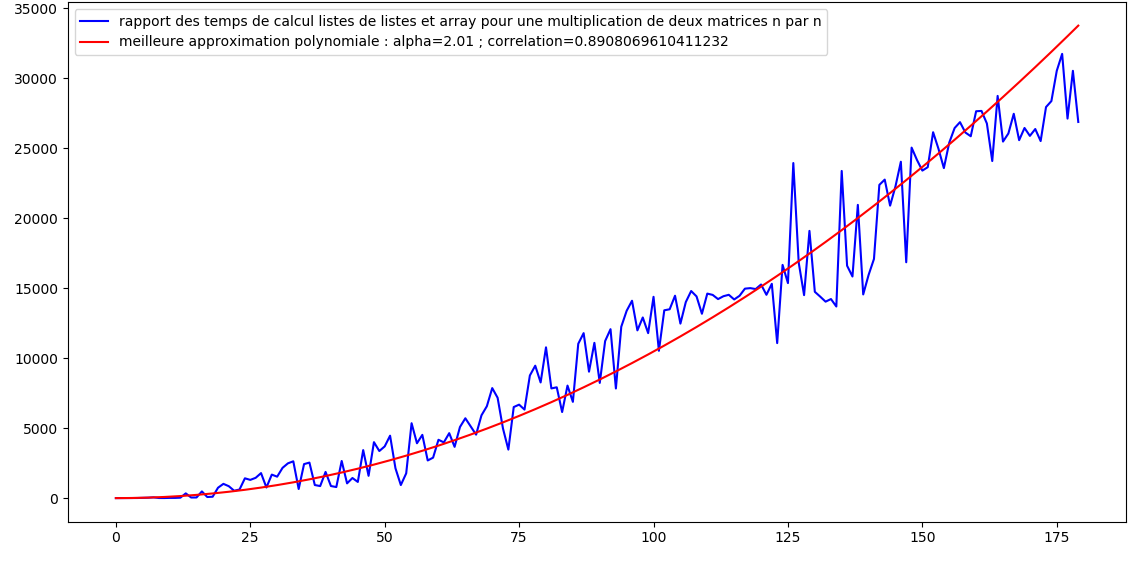
\includegraphics[width=\linewidth]{tpsCalcul.png}
\centering
 \caption{rapports entre le temps de calcul d'une multiplication matricielle avec numpy et en itérant selon la taille $n$ de la matrice. la vitesse est multipliée par  $n^{2}$ }
 \label{fig:tpsCalcul}
\end{figure}


 Chaque équipe a donc tenté lors de cette étape de coder sa version d'un réseau d'apprentissage du XOR, en utilisant pour commencer la fonction d'activation sigmoïde et un apprentissage stochasticque. Malgré la simplicité apparente de cette tâche, les résultats ont divergé, les réseaux n'arrivant pas à classifier correctement tous les cas du XOR s'il avait trop peu de neurones intermédiaires.

Le premier constat fut donc le suivant : L'assurance de la convergence de l'erreur vers $0$ ne se fait que lorsque la couche intermédiaire du réseau a au moins 4 neurones.

Ces résultats nous permettent de vérifier pour ce problème le théorème selon lequel tout problème de classification peut être traité efficacement par un perceptron n'ayant qu'une couche intermédiaire si cette couche est assez grande. la nécessité d'avoir une couche intermédiaire vient pour le cas du XOR, de la non linéarité du problème.

Avant de s'atteler à une application plus complexe, nous avons pris du temps pour tester l'influence de différents paramètres sur la vitesse de convegernce de notre perceptron vers la fonction XOR. 
Nous avons isolé plusieurs hyperparamètres, à savoir  la facon d'initialiser les poids et biais, la vitesse d'apprentissage (ou plus généralement la fonction de minimisation qui pourra ne pas être un gradient simple), la façon de gérer notre set d'entraînement (batch training, stochastich training), la fonction d'activation choisie, ou encore la forme du réseau.

\begin{figure}[H]
\centering
\subfloat[fonction sigmoïde, entrées non centrées]{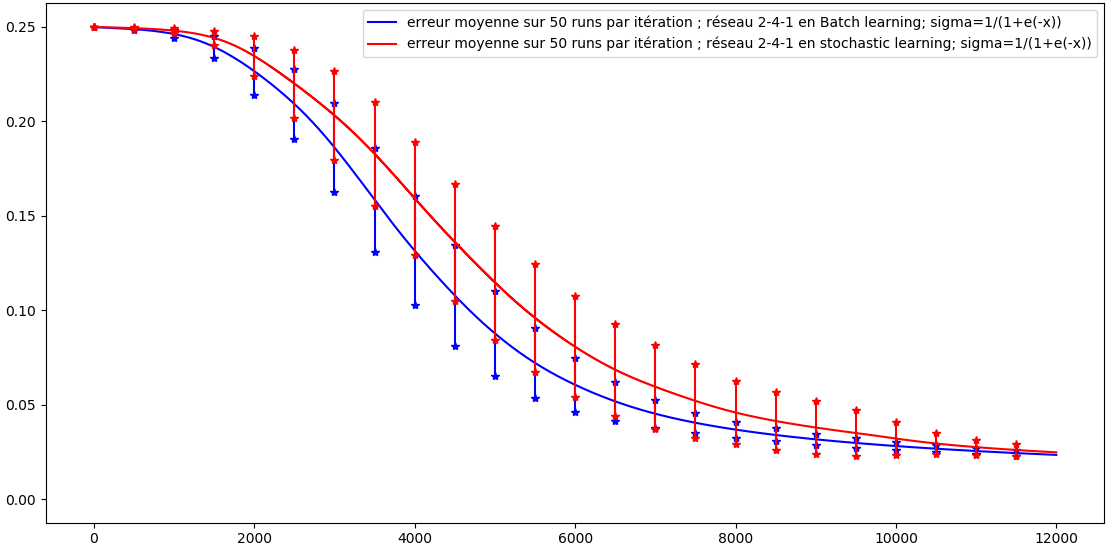
\includegraphics[width=0.49 \linewidth]{XOR41SBSC.png}}
\hspace{1mm}
\subfloat[fonction sigmoïde, entrées centrées]{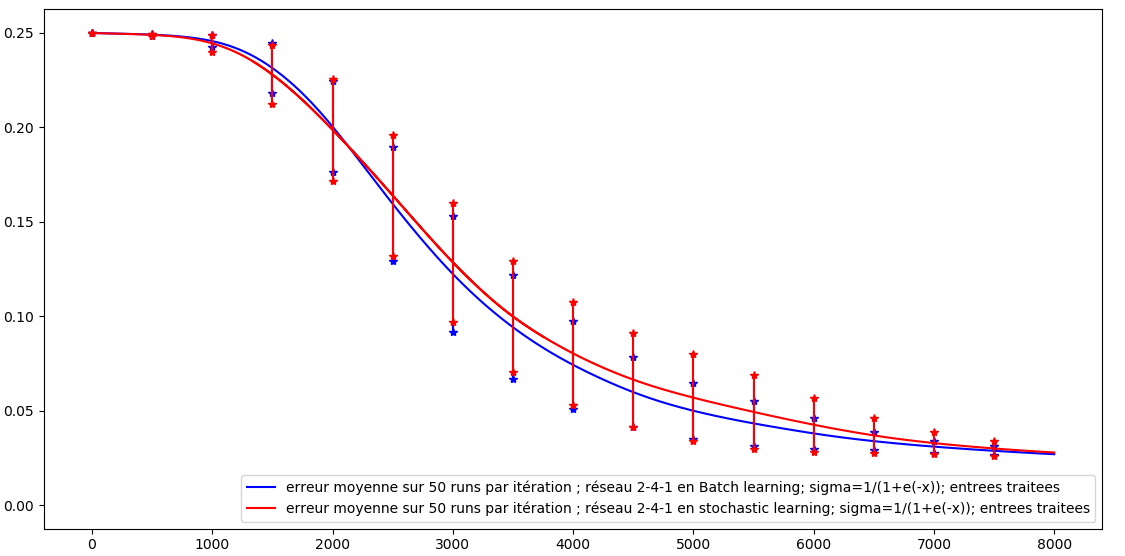
\includegraphics[width=0.49\linewidth]{XOR41SBSCT.png}}
\vspace{2mm}
\subfloat[fonction tanh, entrées non centrées]{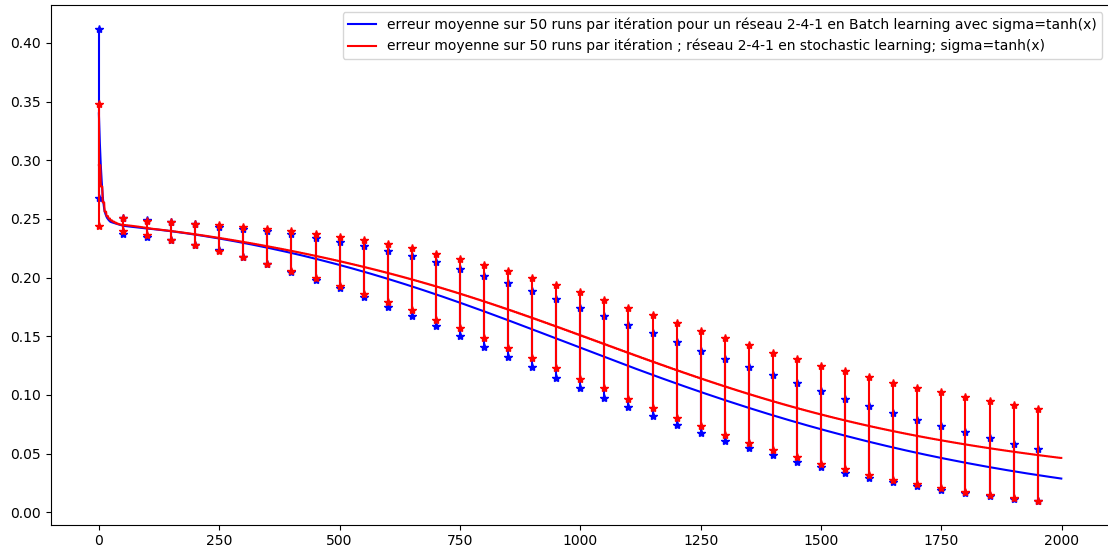
\includegraphics[width=0.49 \linewidth]{XOR41TBSC.png}}
\hspace{1mm}
\subfloat[fonction tanh, entrées centrées]{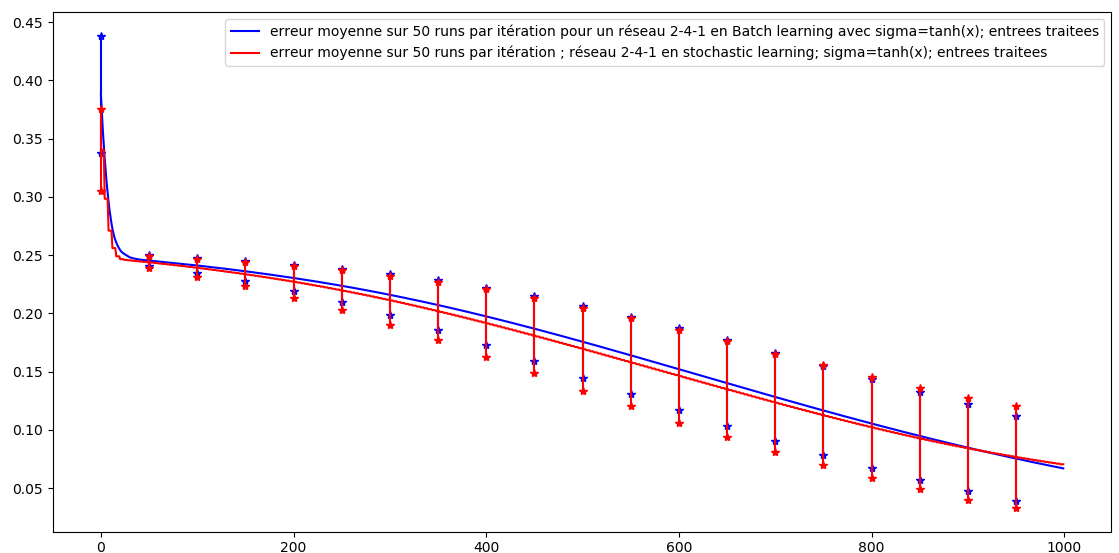
\includegraphics[width=0.49\linewidth]{XOR41TBSCT.png}}

\caption{comparaison du nombre d'itérations pour approximer la fonction XOR avec un réseau 2-4-1 en apprentissage Batch et stochastique selon différents paramètres}
\end{figure}

Nos conclusions nous ont mené, dans la suite de l'étude, à utiliser la fonction tangente hyperbolyque plutot qu'une sigmoïde, à centraliser et réduire les entrées, et à choisir des poids initialisés autour de zéro et des biais initialisés nuls.

\subsection{application au problèmme de classification de chiffres manuscrits}

Le problème classique que l'on a choisi de résoudre avec un réseau de neurones est celui de la classification de chiffres manuscrits. pour cela, on utilise la base de données MNIST, un dataset disponible en ligne comprenant des dizaines de milliers d'images de $28\times 28$ pixels en nuances de gris, chacune représentant un chiffre entre $0$ et $9$, celui-ci étant fourni avec l'image. le perceptron que l'on va utiliser pour classifier l'image aura donc un vecteur d'entrée de taille $784$, et un vecteur de sortie de taille $10$. Dans la suite du rapport, les résultats seront donnés après un léger post-traitement: on choisira pour classifier un nombre, la coordonnée du vecteur de sortie étant maximale, et nos pourcentages de réussites seront fondés sur ce principe.

\begin{figure}[h!]
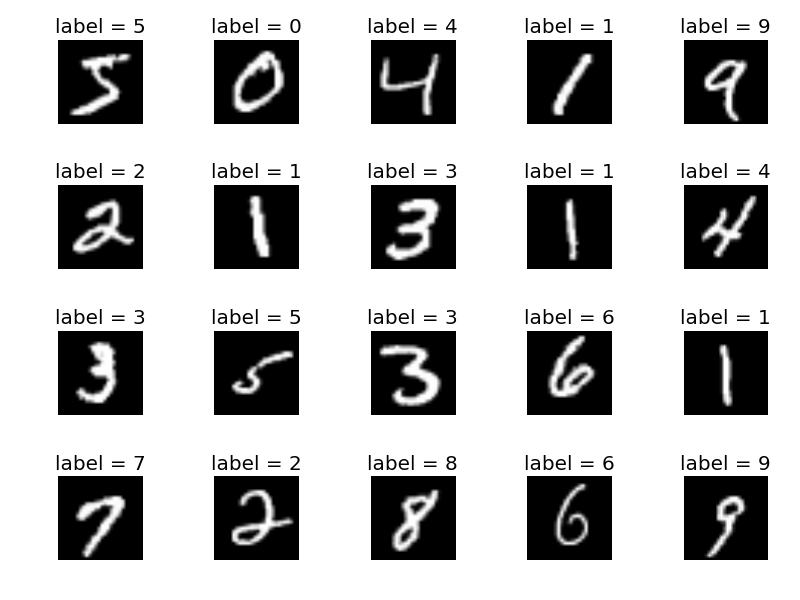
\includegraphics[width=0.8 \linewidth]{MNIST.png}
\centering
 \caption{exemple d'images tirées de la base de données MNIST}
 \label{fig:MNIST}
\end{figure}

La suite consistait alors en la réalisation d'un réseau de neurones pouvant travailler sur la base de de données MNIST des chiffres manuscrits, et sachant à terme reconnaître les chiffres. Le premier souci en terme de travail d'équipe a été rencontré à ce moment-là : deux membres du groupe avaient chacun écrit une version de l'algorithme d'apprentissage, et après discussion tendues, les deux membres ont travaillé ensemble à la réalisation du perceptron. La nécessité d'utiliser les outils de programmation collectives tels GitHub d'une bonne manière s'est fait ressentir.
\vspace{5mm}

Nos perceptrons ont rapidement réussi à résoudre ce problème de classification, mais en regardant plus précisement, les paramètres liés à nos premiers résultats différaient énormément des résultats théoriques, surtout en terme de vitesse de calcul et en taux d'apprentissage : alors qu'il devrait être de l'ordre de $10^{-4}$ pour obtenir une convergence précise et suffisante, nous pouvions monter jusqu'à $10^{-1}$ voire $1$, et toujours converger assez lentement (voir figure 5). Ce problème restera dans notre code sans en trouver de réelle raison pendant environ 1 mois.

\begin{figure}[h!]
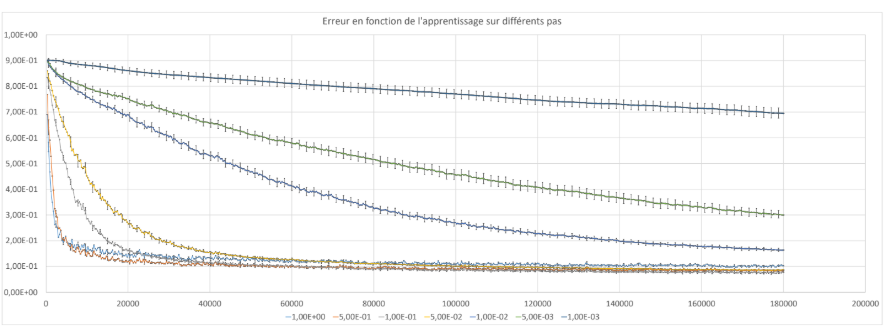
\includegraphics[width=\linewidth]{errorRate.png}
\centering
 \caption{influence du learning rate sur la vitesse de convergence (en nombre d'itérations de l'entraînement) }
 \label{fig:errorRate.png}
\end{figure}

Quant à la vitesse de calcul, elle était grandement affectée par le premier choix que nous avions fait de conserver les formules itératives des calculs de valeurs de neurones. L'équipe Eponge, en parallèle, avait un temps de calcul de l'ordre de la minute là où nous avions un temps de calcul de l'ordre de l'heure. Le passage de la forme itérative à la forme matricielle, pour le calcul des valeurs des réseaux de neurones optimisa grandement le temps de calcul, et est une preuve de l'incroyable efficacité des modules de calcul matriciel de Python. 

\vspace{5mm}
Les valeurs des erreurs finales restant malgré tout satisfaisantes et cohérentes, nous avons donc décidé de travailler sur d'autres facteurs, tels que l'initialisation des paramètres du réseau, et la taille des batch (réduits à 1 élément dans le cas du stochastic training).

Les travaux de LeCun affirmaient que l'initialisation des valeurs des poids et des biais des neurones étaient à rendre aléatoires selon une loi normale centrée. Nous avons donc voulu tester différentes manières d'initialiser ces paramètres, ce qui nous a permis de rapidement exclure l'idée d'initialiser tous les poids à $0$, comme on le voit sur la figure 6. 

\begin{figure}[h!]
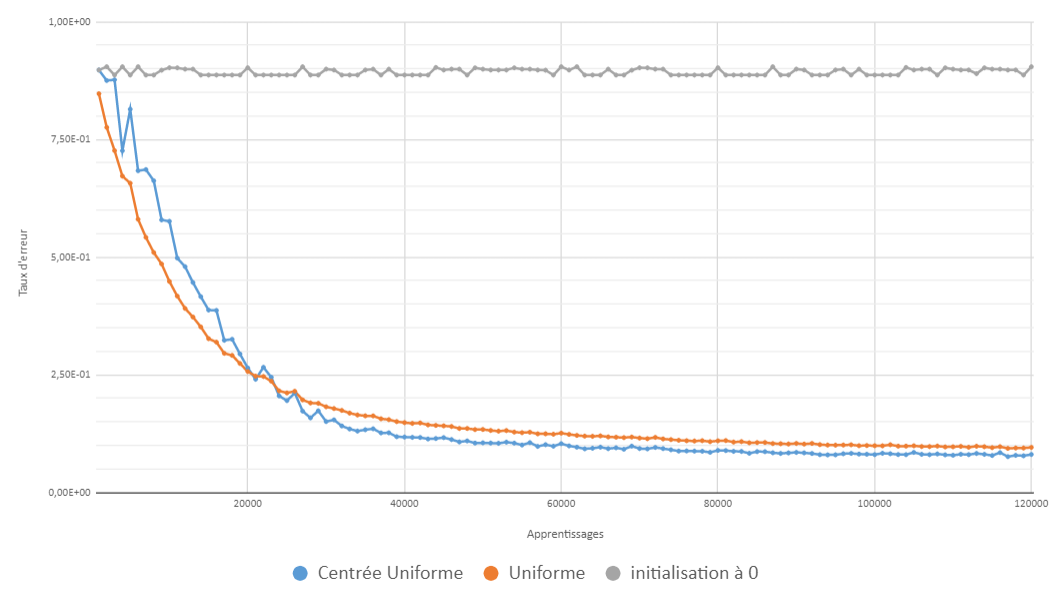
\includegraphics[width=\linewidth]{initPoids.png}
\centering
 \caption{influence de l'initialisation des poids sur la vitesse de convergence (en nombre d'itérations de l'entraînement) }
 \label{fig:initPoids.png}
\end{figure}

Nous avons pour la suite du projet travaillé en "batch-training". Cette méthode d'apprentissage signifie que nous minimisons la fonction de coût selon la moyenne de son expression sur plusieurs entrées du set d'apprentissage, regroupées dans un batch.

La taille du batch, toutefois, était une question différente : des batchs plus petits, soit un modèle tendant vers un descente stochastique de gradient, permet d'augmenter la vitesse de l'apprentissage, mais le choix d'apprendre sur des batchs plus grands permet une plus grande robustesse à d'éventuels mauvaises données d'entraînement et donc de minimiser la fonction à chaque étape dans une direction plus proche de celle du minimum.

La conclusion qui nous est venue est la suivante : le meilleur compromis entre stabilité et précision de l'erreur finale est obtenu pour des batch de taille entre 16 et 32. Ces résultats sont appuyés par plusieurs travaux tiers cités par leCun. % TODO: ref bibliographique 
\vspace{5mm}

Nous avons ensuite rencontré un second problème face au choix d'une nouvelle vitesse d'apprentissage (rappelons que ce paramètre externe au réseau représente la taille du pas vers la minimisation de la fonction de coût que nous effectuons à chaque itération de l'entraînement)

Nous avions, depuis le début, utilisé la fonction d'activation sigmoïde basique $f(x) = \frac{1}{1 + e^{-x}}$ dans chaque neurone de notre réseau, et donc utilisé des vitesses appropriées pour cette fonction.
Néanmoins, au vu de ses meilleurs résultats sur XOR, nous avons voulu changer vers un réseau de neurones utilisant  la fonction d'activation tangente hyperbolique pondérée, $f(x) = 1.7159 \times tanh(\frac{2x}{3})$.

En gardant un learning rate du même ordre, cette transition nous semblait au premier abord inefficace, voire semblait empirer les résultats. En effet, l'erreur de la reconnaissance des chiffres de la base MNIST ne convergeait même pas lors de nos tests avec la nouvelle fonction d'activation. 

En réalité, l'extrême efficacité de cette fonction, suggérée encore une fois par LeCun, associée à nos taux d'apprentissage bien trop élevés, empêchaient la convergence du réseau de neurones: ainsi, en utilisant une descente de gradient simple, il existe un learning rate théorique maximal au delà duquel il est impossible de continuer de converger une fois proche d'un minimum de la fonction. 
 Quelques jours plus tard, le groupe se rendit compte que la même fonction d'activation, avec des taux extrêmement bas, convergeaient à une vitesse fulgurante, voire trop rapide. %en quoi c'est un problème????
\vspace{5mm}

Une des solutions évoquées à cette problématique est de ne pas utiliser une descente de gradient simple avec un learning rate constant mais plutôt diverses méthodes plus complexes (RMSprop, Adam, une descente avec inertie...) qui modifient la vitesse d'apprentissage en fonction de la vitesse d'apprentissage aux étapes précédentes afin d'accélérer autour des zones plates de la fonction et de réduire la vitesse autour des minima.

\vspace{5mm}

\begin{figure}[h!]
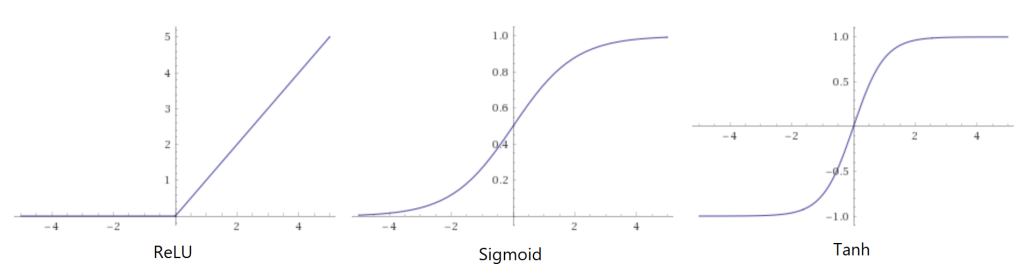
\includegraphics[width=\linewidth]{activations.PNG}
\centering
 \caption{différentes fonctions d'activation pouvant être utilisées dans des réseaux de neurones }
 \label{fig:activations.PNG}
\end{figure}

Enfin, ces fonctions d'activation comportant une zone à pente forte (linéaire) autour de l'origine et une zone à pente faible (saturée) plus l'entrée augmente en valeur absolue, on a rapidement compris, pour augmenter la vitesse de l'apprentissage, l'intérêt de faire en sorte que l'entrée des neurones soit proche de $0$. 

Pour cela, nous avons associé à des poids initiallements centrés et faibles des entrées globales centrées et réduites entre $-1$ et $1$, ce qui a ouvert la voie à la posibilité de réaliser un prétraitement sur les entrées du réseau de neurones plus tard. un prétraitement plus complexe sera utilisé dans la suite. 

\vspace{5mm}
Cette nouvelle efficacité nous a permis de déterminer une toute dernière caractéristique de la base MNIST : sa taille et sa diversité sont si grandes qu'il nous a été impossible d'atteindre l'état de surapprentissage en s'entrainant sur la totalité du set d'entraînement.

Dans le même temps, nous avons rencontré une amélioration concrète de notre vitesse de calcul grâce à la machine virtuelle fournie par nos professeurs encadrants avec l'aide de l'école. L'un des membres de l'équipe disposait également d'une carte graphique NVIDIA 960M, mais au vu de la complexité d'utilisation du CUDA NVIDIA servant aux calculs mathématiques sur carte graphique, la décision a été prise de continuer sur la machine virtuelle.

Toutefois, étant légèrement en retard sur le planning de l'année, et sachant que nos algorithmes réalisaient à peu près ce qui était attendu d'un réseau de neurones, nous sommes passés à l'étape suivante du projet : l'apprentissage de la théorie des réseaux à convolution.
\vfill

\section{Réseaux de neurones à convolutions}


Notre étude des réseaux neuronaux à convolution n'a été dans un premier temps que théorique: l'intérêt n'était pas d'aprendre à en coder un "avec les mains" mais surtout de se renseigner sur le fonctionnement et le rôle des différents paramètres pour pouvoir l'utiliser à bon escient pour résoudre des problèmes pour lesquels c'est un un outil adapté, en particulier l'analyse d'images. Ainsi, lors de notre utilisation future de réseaux à convolutions (ou CNN) fournis par des modules comme tenserflow, nous ne nous retrouvions pas à utiliser l'outil comme une boite noire.
\vspace{5mm}

Les réseaux de neurones à convolutions, comme nous allons le voir, sont souvent utilisés dans l'analyse d'image, car ils compensent le principal problème des perceptrons classiques dans le cas de vecteurs d'entrées de haute dimension: la lenteur de l'apprentissage. En effet, le nombre de poids et donc le nombre de dérivées à calculer va vite trop augmenter : par exemple, si l'on veut classer une image $300\times300$ selon un critère binaire et si $n$ est la taille de la couche intermédiaire, on aurait plus de $90000 n$ paramètres selon lesquels il faudrait calculer la dérivée partielle à chaque itération de l'entraînement, ce qui rendrait l'apprentissage impossible en temps fini. 
\vspace{5mm}
ce problème est résolu par les réseaux à convolutions. La particularité de ce réseau vient du fait qu'entre la couche d'entrée et la couche classique précédent la couche de sortie ( appelée "fully-connected") vont venir plusieurs type de filtres:
\begin{itemize}
	\item des couches de convolutions, qui vont traiter les données reçues avec des filtres fixes. le nombre de filtres sera la troisième dimension de la sortie.
	\item des couches de pooling, permettant de compresser l'information en sortie des couches de convolutions
	\item des couches de corrections, permetant de recentrer les données de sorties par des fonctions d'activations (on utilise souvent ReLu)
\end{itemize}

les caractéristiques recherchées des CNN sont dues au fonctionnement des couches de convolutions : celles-ci vont déplacer une matrice filtre sur l'image d'entrée de manière à obtenir en sortie une image, un point de la matrice de sortie est le résultat de la convolution du filtre ( souvent choisi $3\times3$ ou $5\times5$) par un carré de la matrice d'entrée de même taille.
Ce type de filtrage lui confère les propriétés suivantes :
\begin{itemize}
	\item Premièrement, chaque sortie du filtre ne va plus dépendre de toutes les entrées mais d'un groupes d'entrées proches dans la matrice d'entrée. On va donc introduire la notion de localisation, ce qui va imposer de transmettre le vecteur d'entrée sous une forme adaptée.
	\item Deuxièmement, on peut remarquer que l'association de la convolution avec le ReLU va faire en sorte que l'activation d'un neurone soit uniquement liée à la similarité du groupe de points de l'entrée auquel il correspond avec le filtre, et non de la position de l'entrée: le résultat est invariant par translation.
	\item Enfin, ces propriétés permettent aux CNN d'obtenir une meilleure résistance aux erreurs dans l'estimation des paramètres des filtres puisque, pour un training set fixé, la quantité de données par paramètres est plus grande que pour un MLP. Le partage de poids permet aussi de réduire considérablement le nombre de paramètres à minimiser. On diminue donc les besoin en mémoire et en quantité d'opérations.
\end{itemize}

\begin{figure}[H]
\centering
\subfloat[alternance des couches dans un CNN]{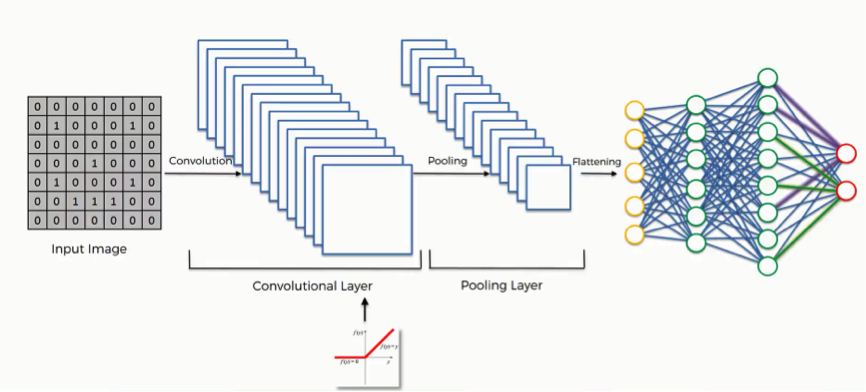
\includegraphics[width=0.49 \linewidth]{couchesCNN.png}}
\hspace{1mm}
\subfloat[une couche de convolutions]{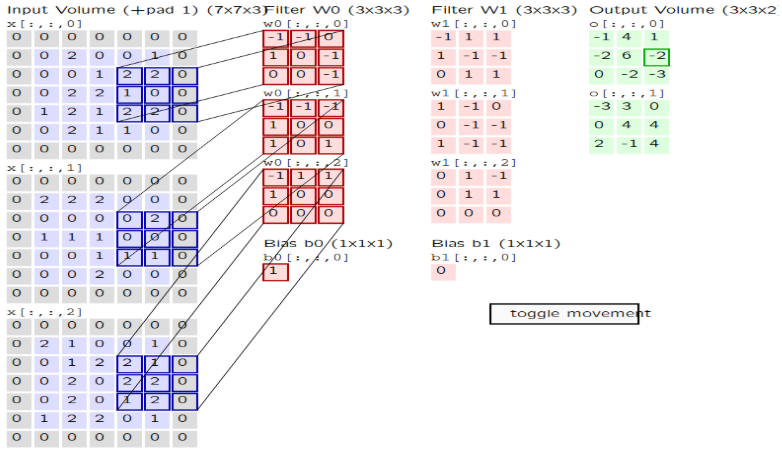
\includegraphics[width=0.4\linewidth]{filtre.png}}
\caption{visualisation du fonctionnement d'un réseau de neurones à convolutions}
\end{figure}


Le CNN va donc s'entraîner à adapter au mieux ses filtres pour pouvoir reconnaître au mieux les motifs (pattern detection) permettant la classification des entrées. comme dans le cas du MLP, nous allons étudier l'influence de plusieurs paramètres sur la vitesse d'aprentissages. 

\subsection{Tensorflow}

Nous avons donc, pour commencer, appliqué un tutoriel basique d'apprentissage sur MNIST, en CNN, fourni par tensorflow. Nous apprendrons plus tard que ce tutoriel utilisait des fonctions obsolètes, nous empêchant de travailler avec tensorboard, l'interface graphique de tensorflow. Toutefois, les résultats en terme d'efficacité de tensorflow étaient bien plus optimisés que nos réseaux neuronaux, et la grande diversité de paramètres nous a introduit à un concept qui ne nous avait pas intéressés jusque-là : le dropout.

Le dropout consiste à désactiver un certain pourcentage de neurones de façon aléatoire (p d'activation du neurone fixé en paramètre). Ce système d'apprentissage " partiel " permet en réalité aux neurones d'être moins dépendants des neurones précédents, et donc plus dépendants de l'entrée en elle-même, mais surtout permet d'éviter le surapprentissage. Toutefois, comme vu auparavant, la base MNIST de par sa taille et sa diversité empêche en elle-même le surapprentissage, ce concept sera donc à garder pour d'autres éventuels systèmes neuronaux.

\begin{figure}[h!]
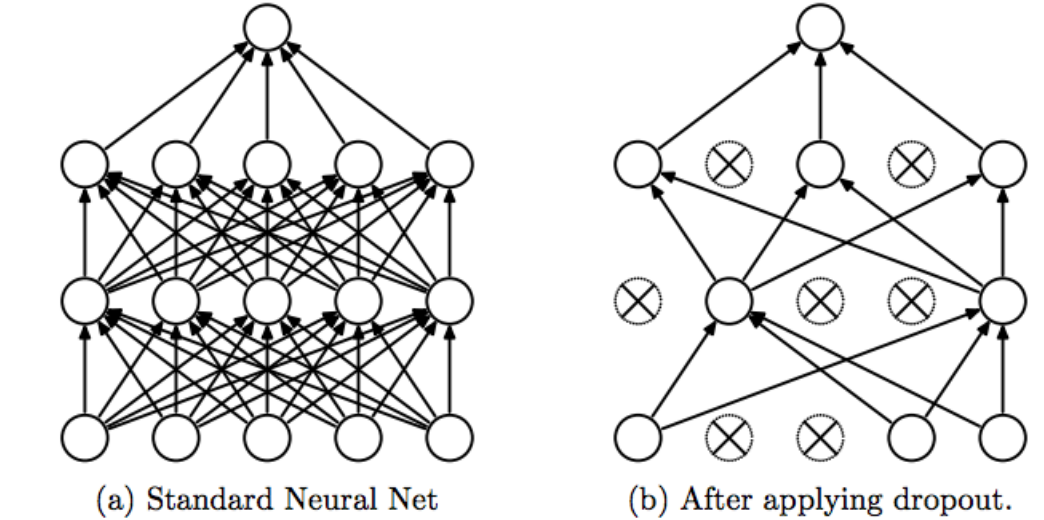
\includegraphics[width=\linewidth]{dropout.PNG}
\centering
\caption{description du dropout dans le cas simple d'un perceptron}
\label{fig:dropout.PNG}
\end{figure}


Nous avons eu l'occasion de discuter avec un ancien élève de Supélec lors de l'une des nombreuses réunions de projet, qui travaillait également avec tensorflow sur de l'analyse de signaux. Cet élève nous a gracieusement fourni un code tensorflow, utilisant des fonctions actuellement à jour, et permettant la visualisation en direct de tensorboard et des différents graphiques liés à nos réseaux de neurones. Si la partie graphique de tensorboard est assez intuitive à prendre en main, la déconcertante complexité du code nécessaire à son bon fonctionnement a été une embûche à notre avancement.

Une fois l'étape des CNN terminée, les profs encadrants nous ont donné pour but de travailler sur le Q-learning : une théorie de l'apprentissage par machine tout à fait différente des perceptrons, avec des cas d'applications tout aussi différents.
\vfill

\section{Q-Learning}

L'objectif du Q-Learning est de calculer une fonction permettant au programme de choisir une action dans un ensemble d'actions $a \in A$ en présence d'un environnement ou état $s \in S$. Pour cela, on définit une fonction $Q: S \times A \rightarrow \mathbb{R}$ qui permet d'estimer la qualité du choix de $a$ dans l'état $s$. Il existe une fonction $R: S \rightarrow \mathbb{R}$ donnant la récompense associée à un état $s$. Cette fonction, qui présente très peu de valeurs non nulles, elle la seule manière d'avoir un retour sur la qualité des choix effectués. Elle annonce notamment les cas d'échec ou de succès pour le programme. Si l'espace d'état est de dimension assez faible, on peut estimer la fonction $Q$ par itérations, en connsaissant toutes les valeurs possibles. Cette fonction est donc définie par ce que l'on appelle une Q-table.
 $$Q(s,a) = (1-\alpha) Q(s,a) + \alpha (r + \gamma max_{a'} Q(s',a') )$$


Le Q-learning s'est avéré plus complexe qu'espéré. 
% TODO: [Go rajouter les images de Loic elles étaient bien]
Nous avons donc décidé d'appliquer cette théorie  à un problème bien plus simple que le but final qu'est Pong. Nous avons donc écrit un algorithme de jeu proche de celui de Nim : un ensemble de 11 batons est présenté à chaque joueur, et chacun son tour, chaque joueur doit retirer 1 ou 2 batons. Le but étant de ne pas retirer le dernier baton.

Nous avons entraîné notre "intelligence" avec différents adversaires : un adversaire jouant "aléatoirement", un adversaire "modéré", un adversaire utilisant la même table d'apprentissage que notre intelligence, et un adversaire parfait. Les résultats sur les courbes d'apprentissages ont suggéré que dans la suite, il serait plus judicieux d'entrainer notre algorithme avec un adversaire modéré, ou dont la difficulté varie dans le temps (un parallèle peut être effectué avec l'apprentissage chez l'être humain : confronter un novice à un expert ne fera pas avancer le novice lors de jeux compliqués).
% TODO: [Courbes sur l'apprentissage des batons]

L'étape suivante fut l'application sur un simili-labyrinthe, très simplifié. Encore une fois, les résultats étaient concluants, et la relative complexité du problème par rapport au jeu de Nim nous a permis pour la première d'introduire dans le Q-learning un réseau de neurones. Nous ne pouvions le faire précédemment car l'entrée de l'algorithme n'était en fait qu'un nombre : le nombre de batons restants. Il était donc impossible de donner "plus" ou "moins" de poids à différentes composantes de l'entrée, puisque celle-ci n'en avait qu'une.

Malheureusement pour notre utilisation, l'état consiste en une image à $160 \times 160$ dimensions. Il est impossible d'énumérer tous les états, et donc de définir la fonction $Q$ par un tableau. On va donc faire appel à un système de réseau de neurones afin d'estimer cette fonction.


L'étude préliminaire théorique du jeu de Pong a révélé plusieurs problématiques propres au jeu de pong :
\begin{itemize}
	\item L'utilisation d'un réseau de neurones est absolument nécessaire : utiliser simplement l'observation comme indexeur d'états donnerait un ensemble d'états possible bien trop grand (position de la balle, des joueurs, changement du score, etc...)
	\item ce réseau de neurones sera a priori un réseau à convolution, puisque la problématique de la detection de "patterns" et de leur positionnement est primordiale en jouant à Pong.
	\item L'utilisation des 3 couleurs (RGB) n'est pas forcément utile, on se limitera par exemple à une combinaison linéaire du rouge et du bleu, qui donnent le plus de contraste entre les différents éléments de l'écran.
\end{itemize}

D'autres problèmes d'un autre genre se sont présentés à nous lors de l'utilisation des différents modules :
\begin{itemize}
	\item Le module atari\_py, module principal de nos travaux, n'est pas compatible avec Windows.
	\item Il semblait au premier abord que le module gym nécessitait absolument une sortie graphique.
	\item La bibliothèque atari de gym n'a que très peu de documentation en ligne : il nous a été nécessaire de regarder le code source, heureusement disponible en libre accès, pour pouvoir manipuler la bilbliothèque.
\end{itemize}

	
Une fois ces quelques problèmes surmontés, les premiers tests d'intelligence artificielle pour pong ont été effectués. Et les résultats sont les suivants :

\paragraph{Semaine du 10 octobre}

La semaine a été consacrée à l'amélioration des premier résultats obtenus sur XOR, mais surtout sur MNIST.

% TODO: Ajouter la référence de ce conseil
L'utilisation de la tangente hyperbolique $f(x) = 1.7159 \times tanh(\frac{2x}{3})$ a permis d'améliorer les résultats, principalement en accélérant les calculs de propagation par rapport à $f(x) = \frac{1}{1 + e^{-x}}$.

Les fonctions permettant de sauvegarder et de charger un perceptron après apprentissage dans un fichier ont été rajoutées. Mais la structure de donnée de l'autre groupe n'est pas forcément identique, il faut donc se mettre d'accord sur un format de fichier commun. Il sera ensuite possible de vérifier le comportement de propagation des deux perceptrons, qui devrait être identique.

\paragraph{Semaine du 30 octobre}

L'équipe a continué à se renseigner sur les réseaux de neurones à convolution. L'accès aux machines virtuelles a permis de lancer des scripts plus longs sans handicaper les membres de l'équipe.

Sur un autre sujet, nous nous sommes penchés sur les différences (de l'ordre d'un facteur 100) entre notre taux d'apprentissage sur MNIST et celui de l'équipe Éponge.

\section{Apprentissage par renforcement}

\paragraph{Semaine du 11 décembre}

Loïc a présenté les premières bases théoriques du Q learning, ou apprentissage par renforcement. Ce genre d'algorithme de machine learning n'est pas utilisé pour des problèmes de classification, mais pour explorer les chemins d'un graphe inconnu, afin de trouver un chemin gagnant (pour une certaine fonction de succès) sans tomber sur un état de défaite.

\paragraph{Semaine du 29 janvier}

Les résultats du Deep Q Learning sur Pong sont décevants. Le modèle semble rapidement converger vers une mauvaise solution, qui fait se bloquer la raquette en haut ou en bas de l'écran. Les scores sont plutôt dus au hasard et sont faibles (défaites 1 ou 2 à 21).

\paragraph{Semaine du 5 février}

L'équipe se met à adapter le code existant concernant le Deep Q Learning sur pong pour une utilisation de tensorflow. En effet, c'est le plus performant pour passer d'un perceptron multicouche à un réseau de convolution. De plus, avec un réseau développé sous tensorflow, il est très facile d'utiliser des cartes graphiques pour décupler les performances.

Lors de la programmation d'un système de Q-Learning, beaucoup de questions qui n'étaient pas à l'ordre du jour pour le développement d'un perceptron entrent en compte. En effet, on se trouve désormais en présence d'un système à apprentissage non supervisé, ce qui diffère grandement à l'entraînement sur les données de MNIST.

\renewcommand{\refname}{\spacedlowsmallcaps{References}} % For modifying the bibliography heading
\bibliographystyle{unsrt}
\end{document}